% ============================================================
%  Marketplace Listings as Routing Interfaces:
%  Auditing Skill Description Adequacy in LLM Agent Ecosystems
%
%  Target: EMNLP 2026 (ARR May cycle)
%  Format: ACL long paper (8 pages + references + limitations)
% ============================================================

\documentclass[11pt]{article}
\usepackage[review]{acl}
\usepackage{times}
\usepackage{latexsym}
\usepackage[T1]{fontenc}
\usepackage[utf8]{inputenc}
\usepackage{microtype}
\usepackage{inconsolata}

% Standard packages
\usepackage{graphicx}
\usepackage{amsmath,amssymb}
\usepackage{booktabs}
\graphicspath{{figures/}}
\usepackage{multirow}
\usepackage{enumitem}
\usepackage{xspace}
\usepackage{xcolor}
\usepackage{hyperref}

% Theorem environments
\newtheorem{observation}{Observation}

% Macros
% System name removed; not used in submission
\newcommand{\clawhub}{\textsc{ClawHub}\xspace}
\newcommand{\skillssh}{\textsc{skills.sh}\xspace}
\newcommand{\eg}{\textit{e.g.,}\xspace}
\newcommand{\ie}{\textit{i.e.,}\xspace}



\title{Do Marketplace Listings Help LLM Agents Choose Skills?\\
Auditing Listing Adequacy in LLM Agent Marketplaces}

\author{Anonymous}

\begin{document}
\maketitle

\begin{abstract}
LLM agents increasingly choose external skills from
marketplace listings that expose only a user-facing
name and description.
We study whether these listings provide enough
information for users and agent routers to understand
a skill before installation.
We define \emph{listing adequacy} and introduce an
Information Completeness taxonomy for apparent
omissions and overclaims.
Using \clawhub---a large open-source agent skill
registry---as a case study, we build an LLM-based
screening auditor calibrated against listing-only expert
judgments and triangulated with implementation-grounded
and programmatic validation.
The audit finds that most listings appear adequate,
while a small subset appear to omit security-relevant or
functional capabilities or overclaim their scope.
Controlled routing experiments across three model families
show modest aggregate disclosure lift (+0.9pp), with
skill names often serving as dominant matching cues.
In a curated OpenClaw name-blind setting, however,
disclosure repair yields +8.1pp routing lift
(95\% CI [1.5, 14.7], $p$=0.015), exposing a
description-dependent failure that aggregate results mask.
Finally, selection experiments show that agents prefer
some functionally similar skills over others, and that
both descriptions and names influence these choices.
Overall, skill listings should be treated as active
inputs to agent retrieval and selection, not as passive
metadata.
\end{abstract}

% ============================================================
\section{Introduction}
\label{sec:intro}
% ============================================================

LLM agents increasingly rely on external skills---web
search, code execution, API integration---to extend
their capabilities~\cite{schick2023toolformer,
qin2023toolllm, patil2023gorilla}.
In marketplace-style deployments, skill selection is
mediated by user-visible natural-language listings:
the name and description that appear before installation.

Unlike API signatures or benchmark tool descriptions,
marketplace listings are author-written, unverified,
and often sparse.
This creates an under-studied dependency: listings
serve as inputs to retrieval, comparison, and
selection, yet their quality is not systematically
assessed.
If a listing omits a capability, that capability may
become difficult for routers to retrieve or select.
If a listing overclaims, users install skills that
cannot deliver.
Strategically written listings may also bias selection.

Prior work has studied tool-calling
accuracy~\cite{schick2023toolformer},
prompt injection~\cite{greshake2023indirect},
agent safety~\cite{debenedetti2024agentdojo},
and tool retrieval~\cite{shi2025toolretrieval},
but typically treats skill descriptions as fixed
ground truth.
We study the complementary question: are marketplace
listings adequate as inputs to retrieval and selection,
and what happens when they are not?

We make three contributions, using \clawhub\ as our
primary case study with \skillssh\ as a descriptive
comparison point.
\emph{First}, we formalize \emph{listing adequacy}
for agent skill marketplaces and introduce an
Information Completeness taxonomy that separates
user-facing screening labels from implementation-grounded
validation
(\S\ref{sec:method}--\ref{sec:audit}).
\emph{Second}, we build and calibrate an LLM-based
screening auditor, then apply it to a large marketplace
snapshot where it classifies 95.0\% of listings as
adequate and flags a small minority for apparent
omissions or overclaims. Routing experiments across
three model families show modest aggregate disclosure
lift (+0.9pp), but a name-blind evaluation isolates a
larger description-dependent effect (+8.1pp; 95\% CI
[1.5, 14.7]; $p$=0.015)
(\S\ref{sec:impact}).
\emph{Third}, we use position-rotated selection
experiments, description swaps, and name/description
ablations to show that agents exhibit stable preferences
among functionally similar skills, with descriptions and
names contributing separable signals
(\S\ref{sec:bias}).
To our knowledge, this is the first large-scale
empirical study focused specifically on user-visible
listing adequacy in an LLM agent skill marketplace.

% ============================================================
\section{Background and Related Work}
\label{sec:background}
% ============================================================

\subsection{Tool-Augmented LLMs and Skill Selection}
\label{subsec:tool_llm}

Modern LLM agents use tool-calling APIs to extend their
capabilities~\cite{schick2023toolformer, qin2023toolllm,
patil2023gorilla}.
In marketplace-style deployments, the agent receives a set of
skill descriptions and must select the appropriate skill for each
user request.
The skill's natural-language description thus becomes the
primary interface between skill authors and the agent's routing
logic, directly determining which skills are retrieved,
compared, and ultimately invoked.
Hsieh et al.~\cite{hsieh2023tool} show that tool documentation
quality directly affects zero-shot tool-use accuracy,
underscoring the importance of description fidelity.

\subsection{Description Quality and Selection Bias}
\label{subsec:desc_quality}

Several lines of work study how tool descriptions affect LLM
tool use.
SkillReducer~\cite{skillreducer2026} addresses missing or
verbose skill descriptions and proposes token-efficient
compression.
BiasBusters~\cite{biasbusters2026} demonstrates that LLMs
exhibit systematic skill selection preferences influenced by
description features.
Compared to these works, we focus on descriptions that are
\emph{present but inadequate}---marketplace listings that
may omit critical information or mislead users about a
skill's true scope, affecting both retrieval and routing.
We extend BiasBusters' methodology to a real marketplace
corpus and analyze which specific description features
correlate with selection.

\subsection{Agent Safety and Tool-Calling Benchmarks}
\label{subsec:safety_bench}

AgentDojo~\cite{debenedetti2024agentdojo},
InjectAgent~\cite{injectagent2024}, and
Yang et al.~\cite{yang2024watch} study skill-level attacks
including prompt injection, backdoors, and data exfiltration,
focusing on risks \emph{after} a skill is selected.
ToolBench~\cite{qin2023toolllm},
API-Bank~\cite{li2023apibank}, and recent tool
retrieval work~\cite{shi2025toolretrieval} evaluate
whether LLMs can invoke the correct tool across large
collections.
However, these benchmarks assume that skill descriptions are
ground-truth and do not study what happens when descriptions
are incomplete or misleading.
Our work fills this gap by treating descriptions as
\emph{variables} rather than constants, and by focusing on
the temporally prior attack surface: the skill
\emph{description} as a pre-installation trust interface
that determines \emph{which} skill is selected in the first
place.
This parallels work on description-to-permission
fidelity in mobile app stores~\cite{felt2011android}
and API ecosystem security audits~\cite{liao2024rapidapi},
but targets the emerging LLM agent marketplace setting.
Figure~\ref{fig:pipeline} summarizes our pipeline.

% ============================================================
\begin{figure*}[t]
  \centering
  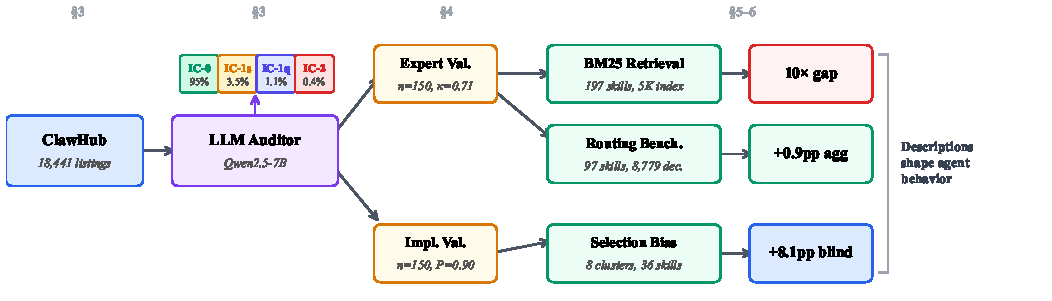
\includegraphics[width=0.95\textwidth]{figures/pipeline_v3}
  \caption{Listing-audit pipeline for the \clawhub\ snapshot
  ($n$=18{,}441 listings). The LLM auditor classifies
  listings along four IC axes, is calibrated against
  listing-only expert labels ($n$=150), and is checked
  with implementation-grounded validation ($n$=150).
  Downstream experiments measure retrieval, routing,
  and selection effects.}
  \label{fig:pipeline}
\end{figure*}
% ============================================================
\section{Listing Adequacy Framework}
\label{sec:method}
% ============================================================

\subsection{Problem Definition}
\label{subsec:adequacy}

Given a skill listing $l = (n, d)$, where $n$ is the
user-visible name and $d$ is the user-visible description,
\emph{listing adequacy} asks whether $l$ provides enough
information for a reasonable user or agent router to
infer the skill's likely scope before installation.
We operationalize ``reasonable user'' as someone with
general technical literacy but no access to the
implementation: can they form correct expectations
about the skill's capabilities, data access, and
side effects from the listing alone?
We distinguish this from implementation correctness:
a listing can be inadequate even if the implementation
is benign and functional.

\paragraph{Scope.}
Our audit evaluates user-visible listing adequacy,
not implementation correctness or malicious intent.
Labels are screening signals for human review;
downstream experiments test effects in controlled
settings and do not estimate deployment-wide rates.

\paragraph{Information Completeness taxonomy.}
We formalize listing adequacy via \emph{Information
Completeness} (IC), shown in Table~\ref{tab:ic_taxonomy}.

\begin{table}[t]
\centering\small
\begin{tabular}{lp{2.9cm}p{2.9cm}}
\toprule
\textbf{Class} & \textbf{User-facing} & \textbf{Implementation-grounded} \\
\midrule
IC-0 & Description conveys the skill's likely scope & Description matches implementation capabilities \\
IC-1s & Description appears to omit security-relevant operations & Implementation contains undisclosed security-relevant operations \\
IC-1q & Description appears to omit functional capabilities & Implementation has features absent from description \\
IC-2 & Description claims capabilities beyond likely scope & Implementation lacks claimed capabilities \\
\bottomrule
\end{tabular}
\caption{IC taxonomy: user-facing definitions (assessed
by our auditor) vs.\ implementation-grounded definitions
(requires implementation-level validation;
see \S\ref{subsec:validation_impl}).}
\label{tab:ic_taxonomy}
\end{table}

Our auditor operates on user-facing definitions only
(left column), inferring \emph{likely} capabilities
from the skill name and category.
The implementation-grounded definitions (right column)
require reading source code and are outside the scope
of our ecosystem-wide audit; we provide a partial
validation on 150 sampled skills
(\S\ref{subsec:validation_impl}).
An omission is labeled IC-1s when it concerns
credentials, network access, file-system modification,
shell execution, or similarly security-relevant
operations; other omissions are labeled IC-1q.

\subsection{Data: Two Agent Marketplaces}
\label{subsec:data}

We study two production marketplaces:

\paragraph{\clawhub.}
We use a commit-level snapshot of a large open-source
agent skill platform.
Each listing includes a user-visible name and optional
description; a subset contains non-trivial implementation
bodies used only for validation
(\S\ref{subsec:validation_impl}).
Our auditor processes the user-visible listing---the
information visible before installation---not the
implementation body.

\paragraph{\skillssh.}
A curated registry aggregating skills from multiple platforms.
Descriptions are substantially longer on average, providing
more surface for both information and manipulation.
We use \skillssh\ for cross-platform comparison only.
Table~\ref{tab:corpus} summarizes the two snapshots.

\begin{table}[t]
\centering\small
\begin{tabular}{lrr}
\toprule
& \textbf{\clawhub} & \textbf{\skillssh} \\
\midrule
Total skills & 18,441 & 116,208 \\
With description & 13,576 & 114,515 \\
Median desc length & 159 chars & 487 chars \\
With non-trivial impl.\ body & 6,912 & --- \\
\bottomrule
\end{tabular}
\caption{Corpus statistics. Although every \clawhub\ entry
contains a \texttt{SKILL.md} file, only a subset contain
non-trivial implementation bodies suitable for
implementation-grounded validation (\S\ref{subsec:validation_impl}).}
\label{tab:corpus}
\end{table}

\subsection{Abstraction Gap}
\label{subsec:abstraction_gap}

A simple lexical approach to detecting description--capability
mismatches would compare code-level patterns
(\eg \texttt{subprocess}, \texttt{os.environ}) against
description keywords
(\eg ``execute shell command,'' ``API key'').
We identify a key limitation of this methodology.

Marketplace descriptions operate at a high semantic level.
Traditional regex detectors flag a \emph{vocabulary mismatch}
between description and code: e.g., ``publishes to WeChat''
does not contain \texttt{subprocess.run()}, so the skill is flagged.
In a pilot study, such flags were overwhelmingly false
alarms: the description was simply operating at a higher
semantic level.
This \emph{abstraction gap} can inflate apparent mismatch
rates by more than an order of magnitude
(Figure~\ref{fig:abstraction_gap}).
The gap shows that listing adequacy cannot be evaluated
by lexical overlap between descriptions and implementation
tokens; the relevant question is whether the listing
conveys the capability at the level users and agents
operate.

\begin{figure}[t]
  \centering
  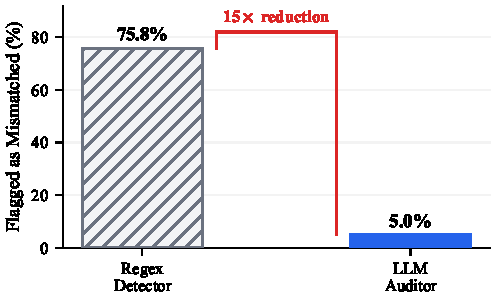
\includegraphics[width=0.68\columnwidth]{figures/abstraction_gap_v2}
  \caption{Abstraction gap: lexical detectors conflate
  vocabulary mismatch with genuine omission, while semantic
  auditing reasons at the user's level.}
  \label{fig:abstraction_gap}
\end{figure}

\subsection{LLM-Based Listing Auditor}
\label{subsec:auditor}

We replace heuristic detectors with an LLM-based auditor
that reduces false positives from lexical mismatch:
it understands that ``publishes to WeChat'' implies
credential handling without requiring the description to
mention \texttt{api\_key} verbatim.

For each skill, the auditor receives the marketplace description
and classifies along four axes:
(1)~IC class (IC-0/IC-1s/IC-1q/IC-2);
(2)~overclaim severity (none/minor/major);
(3)~quality issues (Q1--Q4: missing parameters, vague triggers,
functional overclaim, missing permissions);
(4)~abuse signals (A1--A3: impersonation, concealment, inflation).

The prompt template instructs the auditor to reason as a
\emph{reasonable marketplace user}:
\begin{quote}\small
``You are an auditor for an AI agent skill marketplace.
Given ONLY the skill name and description (what a user sees
before installation), assess whether the description
adequately represents the skill's likely capabilities.''
\end{quote}
The auditor responds with a structured JSON object containing
the IC class, severity, reasons, and confidence score.
We use a structured-rationale prompt that asks the
model to summarize expected capabilities, identify
potential gaps, and output a JSON classification.

\paragraph{Model.}
We use Qwen2.5-7B-Instruct~\cite{qwen2025}, served via
HuggingFace Transformers on a single NVIDIA A100 GPU.
Temperature is set to 0.1 for near-deterministic outputs;
top-p/top-k are not overridden from serving defaults,
inputs are capped at 6k characters, and the full prompt
template is provided in Appendix~\ref{app:prompt}.
The choice of an open-weight model improves reproducibility.

\paragraph{Scope.}
The auditor processes only user-visible listing fields---the
skill name, category, and description visible on the
marketplace before installation.
This represents the ``reasonable user'' perspective:
can a person reading only the marketplace listing understand
what the skill will do?
We deliberately exclude the \texttt{SKILL.md} implementation
file (which users do not typically read before installation)
to avoid conflating developer documentation with
user-facing information.
We acknowledge a tension: the auditor infers \emph{likely}
capabilities from the skill name, which may produce false positives
(e.g., inferring network access for a ``database connector''
that only manages local schemas).
Our validation (Table~\ref{tab:validation}) shows this
manifests as moderate precision for flagged classes,
acceptable for a screening tool but not a ground-truth oracle.

\paragraph{What the audit does not claim.}
The audit does not determine whether a skill is
malicious or whether its implementation is incorrect.
Auditor labels are screening signals, not final
security judgments.

\paragraph{Throughput.}
The audit can be run overnight on a single modern GPU,
making the approach practical as a publish-time screening
step for marketplace operators.

\subsection{Human Validation}
\label{subsec:validation}

To calibrate the auditor, two annotators with experience
in agent-tool systems independently labeled a stratified
sample drawn according to auditor-predicted class.
Annotators were blind to auditor predictions and received
only the skill name, description, and category---the same
information available to the auditor.
A pilot round was used to calibrate the annotation
guideline (reproduced in Appendix~\ref{app:annotation_guide})
before the main labeling.
Disagreements were resolved by discussion to a consensus label.

\emph{Important scope note:} because annotators did not
have access to skill implementations, this validation
measures \textbf{auditor--human agreement under the same
incomplete-information condition} (listing only), not
auditor correctness against implementation ground truth.
Table~\ref{tab:validation} should therefore be read as a
calibration check rather than an accuracy benchmark.

Agreement was substantial between annotators
(Cohen's $\kappa$=0.71) and between
the auditor and the consensus labels. Table~\ref{tab:validation}
reports class-wise precision and recall.

\begin{table}[t]
\centering\small
\begin{tabular}{lccc}
\toprule
\textbf{IC Class} & \textbf{$n$} & \textbf{Precision} & \textbf{Recall} \\
\midrule
IC-0  & 50 & 0.97 \scriptsize{[.88,.99]} & 0.95 \scriptsize{[.85,.98]} \\
IC-1s & 50 & 0.72 \scriptsize{[.58,.83]} & 0.80 \scriptsize{[.67,.89]} \\
IC-1q & 25 & 0.68 \scriptsize{[.48,.83]} & 0.64 \scriptsize{[.45,.80]} \\
IC-2  & 25 & 0.76 \scriptsize{[.57,.89]} & 0.72 \scriptsize{[.52,.86]} \\
\bottomrule
\end{tabular}
\caption{Auditor--expert agreement under the listing-only
condition (same information to both), with 95\% Wilson
confidence intervals. IC-0 agreement is
high; flagged classes show moderate precision, consistent
with screening-tool expectations.
Full annotation guidelines and borderline examples in
Appendix~\ref{app:annotation_guide}.}
\label{tab:validation}
\end{table}

The auditor is most reliable when identifying adequate
listings, while flagged classes are noisier.
This is appropriate for screening: flagged listings should
receive human review rather than automatic enforcement.

\paragraph{IC-0 false-negative estimation.}
Among 50 auditor-labeled IC-0 skills in the
implementation-grounded validation, all 50 were classified as
adequate by LLM-derived implementation inspection
(0 false negatives; Wilson 95\% CI upper bound: 7.1\%).
Among sampled implementation-inspectable IC-0 skills,
this suggests the auditor's IC-0 label is conservative.
Extrapolating to the full corpus should be done cautiously:
the upper bound of approximately 1,250 listings among
17,526 IC-0 entries assumes the inspectable sample is
representative, and a larger random sample with human
code audit would narrow this estimate.

% ============================================================
\section{Ecosystem-Wide Audit}
\label{sec:audit}
% ============================================================

We apply the auditor to the full \clawhub\ snapshot.
Table~\ref{tab:ic_dist} summarizes the resulting screening
labels.

\begin{table}[t]
\centering\small
\begin{tabular}{lrr}
\toprule
\textbf{IC Class} & \textbf{N} & \textbf{\%} \\
\midrule
IC-0 (adequate)         & 17{,}526 & 95.0 \\
IC-1s (apparent sec.\ omission)  & 643      & 3.5 \\
IC-1q (apparent func.\ omission)& 196      & 1.1 \\
IC-2 (apparent overclaim)       & 72       & 0.4 \\
Unparseable                     & 4        & $<$0.1 \\
\midrule
Total                   & 18{,}441 & 100 \\
\bottomrule
\end{tabular}
\caption{Auditor-estimated listing adequacy for the
full \clawhub\ snapshot ($n$=18{,}441 listings),
calibrated against listing-only expert labels in
Table~\ref{tab:validation}.
Corpus-level prevalence may differ because validation
was stratified (see \S Limitations).}
\label{tab:ic_dist}
\end{table}

\begin{observation}
\textbf{Most listings appear adequate under auditor screening.}
The large majority of listings are classified IC-0, and
stratified validation shows that this class is reliable.
In contrast, regex-based detection substantially overstates
mismatch because it confuses abstraction with omission.
Among no-description listings, the auditor still classifies
88.2\% as IC-0 (Table~\ref{tab:ic_detailed}) because
the skill \emph{name} alone often conveys sufficient scope
(\eg \texttt{gmail}, \texttt{web-search}).
This reflects the taxonomy design: IC-0 requires only that
a reasonable user can form correct expectations from the
listing as a whole, not that every field be populated.
\end{observation}

\begin{observation}
\textbf{A small subset is flagged for apparent omissions.}
The auditor flags a small minority of listings for apparent
security-relevant or functional omissions.
These are screening rates rather than final prevalence
estimates; we partially validate them against implementation
bodies in \S\ref{subsec:validation_impl}.
\end{observation}

\paragraph{Cross-platform context.}
\skillssh\ descriptions are longer than \clawhub{}
descriptions, giving authors more room for both useful
detail and manipulative text.
This supports a hypothesis about length and adversarial
surface area, but does not establish causality.

\paragraph{Severity distribution.}
Table~\ref{tab:severity} shows the joint distribution of
IC class and maximum auditor-assigned severity.
Major-severity IC-1s listings are the highest-priority
targets for human review because they appear to omit
security-relevant operations.

\begin{table}[t]
\centering\small
\begin{tabular}{lrrr}
\toprule
\textbf{IC Class} & \textbf{None} & \textbf{Minor} & \textbf{Major} \\
\midrule
IC-0  & 17,449 & 77 & 0 \\
IC-1s & 0 & 547 & 96 \\
IC-1q & 0 & 170 & 26 \\
IC-2  & 0 & 61  & 11 \\
\midrule
\textbf{Total} & 17,449 & 855 & 133 \\
\bottomrule
\end{tabular}
\caption{Joint distribution of IC class and maximum severity
per skill. Major-severity IC-1s listings are the
highest-priority audit targets.}
\label{tab:severity}
\end{table}

\paragraph{Qualitative examples.}
IC-1s listings span diverse categories: e.g., a
messaging skill not mentioning credential handling,
or a data-access skill not mentioning network access.
IC-2 listings include overclaimed capabilities such as
``security scanning'' that describes only API wrapping.

\subsection{Implementation-Grounded Validation}
\label{subsec:validation_impl}

To partially address the gap between listing-level and
implementation-level assessment, we sample skills
stratified by inferred IC class and compare auditor
classifications against
LLM-assisted capability extraction from \texttt{SKILL.md}
implementation bodies.

For each skill, an independent LLM (separate from the
listing auditor) reads the full \texttt{SKILL.md}
implementation body and extracts implementation-level
capabilities---shell execution, credential access, network
calls, and file-system modification.
The implementation annotator is blinded to the listing
auditor's IC label.
We then compare: (1)~the listing auditor's IC class
(based on name+description only) against (2)~the
implementation-derived label.

\paragraph{Results.}
Implementation-grounded validation supports the main
screening result: most auditor-flagged labels are
also supported when the implementation body is inspected.
The false positives mainly arise when a skill name implies
broader scope than the implementation delivers, consistent
with the inherent tension of inferring capabilities from
listings alone.
The full confusion matrix is reported in
Appendix~\ref{app:impl_validation}.

\emph{Caveat:} this validation uses LLM-based capability
extraction from \texttt{SKILL.md} text, not manual code
audit. The verification chain is therefore
\emph{LLM auditor $\to$ LLM implementation extractor},
with no human-verified ground truth in the loop.
The programmatic audit below partially addresses this gap,
but a larger manual audit would further strengthen
these estimates.

\subsection{Programmatic Capability Verification}
\label{subsec:human_impl_audit}

To provide lower-bound supporting evidence independent of
any LLM, we run a regex-based capability detector over
the raw implementation files of 67 IC-1s skills from
our routing benchmark.
Unlike the abstraction-gap analysis in
\S\ref{subsec:abstraction_gap}, which showed that
regex overstates mismatches at the corpus level,
here we use regex conservatively: we only count
a capability as \emph{supported} when the code
contains direct evidence (e.g., literal
\texttt{subprocess} calls), accepting that we will
miss capabilities expressed through abstractions.
For each of five capability types---shell execution,
credential access, network access, filesystem operations,
and email---we search for concrete code-level indicators
(e.g., \texttt{subprocess}, \texttt{API\_KEY},
\texttt{requests.}, \texttt{open(}, \texttt{smtp}).
We compare detected capabilities against description
mentions to identify programmatically supported omissions.

\begin{table}[t]
\centering\small
\begin{tabular}{lrrr}
\toprule
\textbf{Capability} & \textbf{Flagged} & \textbf{Supported} & \textbf{Support rate} \\
\midrule
Shell execution   & 53 & 45 & 84.9\% \\
Credential access & 28 & 21 & 75.0\% \\
Network access    & 35 & 17 & 48.6\% \\
Filesystem        & 19 &  4 & 21.1\% \\
Email             &  9 &  9 & 100\% \\
\midrule
\textbf{Overall}  & \textbf{144} & \textbf{96} & \textbf{66.7\%} \\
\bottomrule
\end{tabular}
\caption{Programmatic verification of auditor-flagged
capability omissions (67~IC-1s skills).
``Flagged'' = description lacks mention but name or
context suggests the capability;
``Supported'' = implementation code contains concrete
evidence. Overall support rate is 66.7\%; 76\% of skills
have $\geq$1 programmatically supported omission.}
\label{tab:programmatic_verification}
\end{table}

Table~\ref{tab:programmatic_verification} shows that
66.7\% of flagged omissions are supported by
implementation evidence, and 76\% of skills (51/67)
have at least one programmatically supported omission.
Shell execution and credential access show high precision
(75--85\%), while filesystem detection is noisier due to
broad pattern matching.
These results are conservative: regex detection misses
capabilities expressed through framework abstractions
(e.g., a skill using a database ORM rather than raw
\texttt{open()} calls).

% ============================================================
\section{Impact on Retrieval and Routing}
\label{sec:impact}
% ============================================================

\subsection{Lexical Discoverability Experiment}

\paragraph{Setup.}
We measure how description sparsity affects lexical
discoverability.
We sample skills with short descriptions and substantive
implementation bodies, which provide a stress-test set for
vocabulary mismatch, and embed them in a large BM25 index.
For each skill we generate \emph{goal} queries
(\eg ``I need to manage database connections'') and
\emph{scenario} queries
(\eg ``My system requires automated report generation'')
from body vocabulary, measuring
Recall@10 under original vs.\ augmented descriptions
(body-derived disclosure sentences added).
Statistical significance is assessed separately for goal
and scenario queries using paired tests; implementation
details are provided in Appendix~\ref{app:retrieval}.
We use BM25Okapi~\cite{robertson2009bm25} with default
parameters ($k_1 = 1.5$, $b = 0.75$).

\emph{Design note}: Queries are drawn from body vocabulary,
so the measured gain is a lexical upper bound;
real user queries may yield smaller gains.
Table~\ref{tab:bm25} reports the results.

\begin{table}[t]
\centering\small
\begin{tabular}{lccc}
\toprule
\textbf{Query type} & \textbf{Original} & \textbf{Augmented} & \textbf{$p$} \\
\midrule
Goal     & 58.5\% & 65.1\% (+6.6pp) & $<$0.001 \\
Scenario & 72.1\% & 75.0\% (+2.9pp) & 0.013 \\
\bottomrule
\end{tabular}
\caption{BM25 Recall@10 under original vs.\ augmented
listings ($n$=197 skills embedded in a 5K-skill index).
Deltas are +6.6pp (95\% bootstrap CI [1.0, 12.4])
for goal queries and +2.9pp (CI [$-$2.2, 7.8]) for scenario
queries. Query generation makes this a lexical
stress test rather than a deployment prevalence estimate.}
\label{tab:bm25}
\end{table}

\begin{observation}
\textbf{Sparse listings reduce lexical discoverability.}
Augmenting listings with capability vocabulary improves
Recall@10 in this stress test, especially for goal-style
queries. Because queries are generated from implementation
vocabulary, the result should be read as an upper bound on
real-world lexical gains.
\end{observation}

\subsection{Routing Repair Experiment}
\label{subsec:routing_gap}

\paragraph{Research question.}
Do IC-1 capability--description mismatches cause
measurable routing failures, and do targeted disclosure
repairs close them?

\paragraph{Experimental design.}
We construct a routing benchmark at two scales.
A small pilot tests feasibility; a larger replication
tests generalizability across skill types, description
conditions, and router models.

For each skill, we generate four query types.
\emph{Description-mentioned} queries reference capabilities
explicitly stated in the listing.
\emph{Undisclosed-capability} queries reference capabilities
present in the implementation but absent from the listing.
\emph{Name-blind} queries describe undisclosed capabilities
without any vocabulary related to the skill name,
isolating the description signal from name-based matching.
\emph{Unsupported-capability} queries target capabilities
the skill does not have (expected rejection).
Each query is evaluated under 4 description conditions:

\begin{enumerate}[nosep,leftmargin=1.2em]
  \item \textbf{Original}: the marketplace description
        as-is.
  \item \textbf{Targeted disclosure}: one sentence appended
        disclosing the omitted capability
        (\eg ``Requires an API key and can read local files'').
  \item \textbf{Length-matched control}: one sentence of
        equal length but irrelevant content
        (\eg ``Plan carefully and review changes early''),
        isolating length from semantic contribution.
  \item \textbf{Structured repair}: a
        Capabilities/Permissions/Limitations template.
\end{enumerate}

The large-scale benchmark contains 97 target skills from
the \clawhub\ corpus: 78 auditor-flagged IC-1 skills
(IC-1s/IC-1q) and 19 IC-0 controls, selected using
manifest-declared permissions cross-referenced against
description text. The IC-1 subset covers apparent security
and functional omissions; the IC-0 controls prevent the
benchmark from containing only omission-positive targets.
Skills are stratified across common omission types
such as shell access, API keys, file-system access,
browser automation, OAuth, email, and collaboration
platforms.
Each routing prompt places the target skill among
distractors drawn from popular skills, using
description-only presentation with deterministic
target positioning for reproducibility.
We evaluate three routers---OpenClaw (default gateway),
GPT-5.4-mini, and Gemini~2.5~Flash---to test whether
findings generalize across model families.

\paragraph{Pilot results.}
The pilot shows the expected asymmetry: queries that
match the listing route reliably, while queries that
depend on omitted capability vocabulary are much more
fragile. Disclosure repair removes this gap in the
pilot setting, motivating the larger benchmark below.

\paragraph{Large-scale results.}
Table~\ref{tab:routing_benchmark} reports routing
accuracy across all 4 conditions and 3 routers.

\begin{table}[t]
\centering\small
\resizebox{\columnwidth}{!}{%
\begin{tabular}{llcccc}
\toprule
\textbf{Router} & \textbf{Condition}
  & \textbf{Original}
  & \textbf{Disclosed}
  & \textbf{Length ctl}
  & \textbf{Structured} \\
\midrule
OpenClaw     & Accuracy & 82.5 & \textbf{83.5} & 82.5 & 82.6 \\
GPT-5.4-mini & Accuracy & 83.7 & 83.7 & 82.2 & 82.8 \\
Gemini 2.5 Flash & Accuracy & 75.8 & 77.6 & 76.0 & 78.0 \\
\midrule
\multicolumn{2}{l}{\emph{Mean disclosure lift}}
  & \multicolumn{4}{r}{\textbf{+0.9pp} (range 0.0 to +1.8)} \\
\bottomrule
\end{tabular}}
\caption{Overall routing accuracy (\%) by condition and
router (97 target skills: 78~IC-1 plus 19~IC-0 controls;
8,779~valid decisions across 3 routers).
Targeted disclosure changes overall accuracy by +1.0pp
for OpenClaw, +0.0pp for GPT-5.4-mini, and +1.8pp for
Gemini; these aggregate effects are descriptive, with the
pre-specified name-blind contrast tested in
Table~\ref{tab:blind_routing}.}
\label{tab:routing_benchmark}
\end{table}

Across all three routers, overall positive-query accuracy
is high (75.8--83.7\%).
For description-trigger queries, original-condition recall
is 94.4\%, suggesting that stated capabilities route
reliably in this benchmark.
Disclosure lift is modest at the aggregate level because
\emph{informative listing text already suffices for most
skills}: 67/78 IC-1 target skills (85.9\%) are routed
correctly by a majority of original-condition decisions.
The isolated description-dependent impact of repair is
masked by this high baseline.

\paragraph{Name-blind analysis.}
To isolate the description signal from name-based matching,
we construct \emph{name-blind} queries that describe
undisclosed capabilities without referencing the skill name
or its synonyms (43 IC-1 skills, 516 routing decisions).
Table~\ref{tab:blind_routing} shows the key result.

\begin{table}[t]
\centering\small
\begin{tabular}{lccc}
\toprule
\textbf{Condition}
  & \textbf{Desc-trigger}
  & \textbf{Body-trigger}
  & \textbf{Name-blind} \\
\midrule
Original            & 90.7 & 89.5 & 90.7 \\
Targeted disclosure & 90.7 & 90.7 & \textbf{98.8} \\
\midrule
\emph{Disclosure $\Delta$} & 0.0 & +1.2 & \textbf{+8.1} \\
\bottomrule
\end{tabular}
\caption{Routing recall (\%) by query type and condition
(43~IC-1 skills, OpenClaw router).
When queries avoid skill-name vocabulary (name-blind),
the disclosure lift is \textbf{+8.1pp}---about 6.8$\times$
the name-containing body-trigger lift (+1.2pp).
This indicates that skill names mask the routing
deficit caused by incomplete descriptions.}
\label{tab:blind_routing}
\end{table}

The disclosure lift is about 6.8$\times$ larger for name-blind
queries (+8.1pp; 95\% CI [1.5, 14.7]; $p$=0.015, $n$=86
per condition) than for standard body-trigger queries
(+1.2pp), and 9$\times$ larger than the aggregate
result (+0.9pp).
In the large-scale name-avoidant benchmark across all
three routers, mean lift is +1.1pp (OpenClaw $-$1.3pp,
GPT-5.4-mini +1.9pp, Gemini~2.5~Flash +2.8pp)
(Appendix~\ref{app:cross_router}), directionally
consistent but smaller than the curated name-blind
result, likely because the large-scale queries
include skills with moderately informative names.
For the 4 skills with fully opaque names ($n$=4; \eg
\texttt{nano-banana-pro}), name-blind recall jumps
from 0\% to 100\% under disclosure---an illustrative
(but small-sample) complete recovery.

\begin{observation}
\textbf{Skill names dominate routing; description gaps
are masked until name signals are removed.}
Aggregate disclosure lift (+0.9pp) underestimates the
isolated description-dependent impact of repair.
When name-based matching is controlled via name-blind
queries, the lift rises to +8.1pp, and skills with
opaque names show 0\%$\to$100\% recovery.
\end{observation}

\paragraph{Query constructedness caveat.}
All queries in both the aggregate and name-blind benchmarks
are synthetically generated from implementation vocabulary
or repair sentences.
This design is appropriate as a diagnostic stress test:
it measures the \emph{diagnostic upper bound} of the routing impact of
description gaps.
However, it may overestimate effects relative to
natural user queries, which may not precisely target
omitted capabilities.
Future work should validate with externally authored
task descriptions.
Figure~\ref{fig:routing_repair} summarizes the
aggregate routing results across all conditions.

\begin{figure}[t]
  \centering
  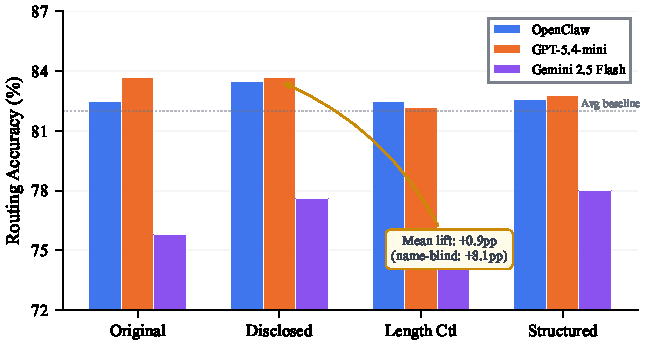
\includegraphics[width=0.95\columnwidth]{figures/routing_repair}
  \caption{Routing accuracy across 4 description conditions
  and 3 routers. Targeted disclosure yields a modest
  aggregate lift, but the effect is masked by skill-name
  signals---see Table~\ref{tab:blind_routing} for the
  name-controlled analysis.}
  \label{fig:routing_repair}
\end{figure}

\paragraph{Comparison with SkillReducer.}
SkillReducer~\cite{skillreducer2026} proposes description
\emph{compression} to reduce token costs.
Our routing benchmark (Tables~\ref{tab:routing_benchmark}
and~\ref{tab:blind_routing})
reveals a complementary problem: IC-1 descriptions
can omit capability vocabulary that routing depends on.
Critically, this gap is \emph{masked} at the aggregate level
by skill names that serve as strong routing cues; it
emerges clearly only in the name-blind evaluation.
Losslessly compressing an incomplete description preserves
the same routing failure---compression cannot repair
a semantic gap.
Description repair (augmentation) and compression
are orthogonal interventions that should be applied
sequentially.

% ============================================================
\section{Selection Bias in Listings}
\label{sec:bias}
% ============================================================
This section asks whether agents show stable skill
preferences, which listing features correlate with
selection, and whether descriptions and names provide
separable signals.

\subsection{Controlled Selection Benchmark}
\label{subsec:benchmark}

\paragraph{Setup.}
Following BiasBusters~\cite{biasbusters2026}, we curate
clusters of functionally similar skills from \clawhub\
and ask LLM agents to choose among them under rotated
presentation orders.
This lets us distinguish skill-level preference from
position bias.
We construct multiple clusters and evaluate them with
cyclic position rotations across models; full cluster
sizes, model configurations, and call counts are reported
in Appendix~\ref{app:bias}.
We measure two concentration scores: \emph{skill-level
concentration} ($\delta_\text{skill}$) captures whether the
model repeatedly selects the same skill, while
\emph{position-level concentration} ($\delta_\text{pos}$)
captures whether it repeatedly selects the same list
position.
A score of 0 means selections are perfectly uniform;
a score near 0.8 means one skill receives nearly all
selections.
Formally,
\[
\delta_\text{skill} = \frac{1}{2} \sum_{i=1}^{K} |p_i - 1/K|
\]
where $p_i$ is the selection proportion of skill $i$ and $K$
is the cluster size; $\delta_\text{pos}$ is defined analogously
over presentation positions.
Table~\ref{tab:bias} reports results across all clusters.

\begin{table}[t]
\centering\small
\begin{tabular}{lccc}
\toprule
\textbf{Cluster} & $\delta_\text{skill}$ & $\delta_\text{pos}$ & \textbf{Top-1 (\%)} \\
\midrule
github\_mgmt   & 0.800 & 0.000 & GitHub (100) \\
image\_gen     & 0.800 & 0.000 & Flux Image (100) \\
video\_gen     & 0.800 & 0.000 & Google Veo (100) \\
memory\_sys   & 0.800 & 0.137 & Cognitive Mem. (100) \\
speech\_to\_txt & 0.600 & 0.000 & Speech To Text (80) \\
twitter\_x    & 0.552 & 0.076 & X Articles (71) \\
text\_to\_speech & 0.400 & 0.000 & Mac TTS (40) \\
web\_search   & 0.400 & 0.000 & Tavily (40) \\
\midrule
\textbf{Mean} & \textbf{0.644} & \textbf{0.027} & --- \\
\bottomrule
\end{tabular}
\caption{Selection concentration by cluster under cyclic
position rotation.
Skill-level concentration ($\delta_\text{skill}$) is
consistently higher than position-level concentration
($\delta_\text{pos}$), suggesting that list order is
not the main source of preference.
Experimental details are reported in Appendix~\ref{app:bias}.}
\label{tab:bias}
\end{table}

\begin{observation}
\textbf{Agents show stable skill preferences after
position rotation.}
Skill-level concentration is consistently higher than
position-level concentration, indicating that preferences
are not primarily an artifact of list order.
\end{observation}

\begin{figure}[t]
  \centering
  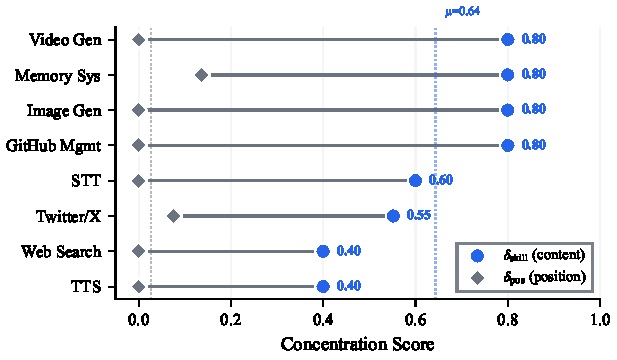
\includegraphics[width=0.95\columnwidth]{figures/selection_concentration}
  \caption{Selection concentration by cluster.
  Skill-level concentration ($\delta_{\text{skill}}$, blue)
  is consistently high across clusters,
  while position-level concentration ($\delta_{\text{pos}}$,
  gray) is near zero, indicating content-driven preference.}
  \label{fig:selection_concentration}
\end{figure}

Figure~\ref{fig:selection_concentration} visualizes
these concentration scores across all clusters.

\subsection{Exploratory Description Feature Analysis}

\begin{table}[t]
\centering\small
\begin{tabular}{lrl}
\toprule
\textbf{Feature} & \textbf{$r$} & \textbf{Interpretation} \\
\midrule
Specificity       & $+$0.654 & Concrete details help \\
Readability (FK)  & $-$0.526 & Simpler text helps \\
Mentions AI/LLM   & $-$0.397 & AI keyword hurts \\
Name length        & $-$0.340 & Shorter names help \\
Promo word count   & $-$0.090 & Not predictive \\
\bottomrule
\end{tabular}
\caption{Pearson correlation between description features
and selection rate ($n$=36 skills, $R^2$=0.52
for combined exploratory linear regression).
\emph{Caveat:} the sample is small and correlations are
exploratory; they should not be interpreted causally.
Leave-one-cluster-out analysis
preserves the sign of the top two features; because the
analysis is exploratory and cluster-confounded, we do not
use these correlations for confirmatory hypothesis tests.}
\label{tab:features}
\end{table}

\begin{figure}[t]
  \centering
  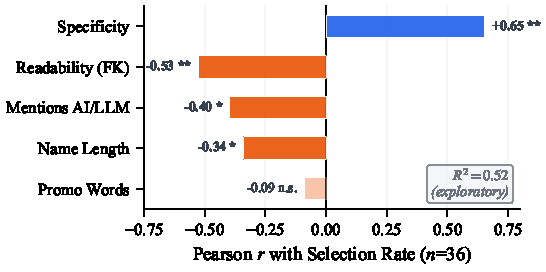
\includegraphics[width=0.85\columnwidth]{figures/feature_correlation}
  \caption{Pearson correlation between description features
  and selection rate. Specificity is the strongest positive
  predictor; promotional language is not predictive.
  The analysis is exploratory and should not be read causally.}
  \label{fig:feature_corr}
\end{figure}

Figure~\ref{fig:feature_corr} visualizes these correlations.

\begin{observation}
\textbf{Concrete and readable descriptions correlate with
higher selection rates (exploratory).}
The strongest correlates of selection are specificity
and readability; promotional language shows little
benefit (Table~\ref{tab:features}).
These correlations are exploratory and may be confounded
by cluster, brand, or capability type; the causal
evidence comes from the swap and ablation experiments
below.
\end{observation}

\paragraph{Preferred vs.\ excluded skills.}
Top-selected skills share concrete capability language,
shorter names, and simpler descriptions.
Excluded skills exhibit vague or circular descriptions.

\paragraph{Qualitative patterns.}
Manual inspection shows that top-selected skills
use concrete action verbs and quantitative details,
while bottom-selected skills use circular definitions
or promotional language without specifics.

\subsection{Automated Description Repair}
\label{subsec:repair}

While BiasBusters~\cite{biasbusters2026} proposes
output-side mitigation, we test \emph{input-side repair}:
rewriting descriptions to start with concrete verbs,
include quantitative details, and simplify language
(full examples in Appendix~\ref{app:repairs}).

\paragraph{Live validation.}
In the \emph{description-swap} condition, we exchange
descriptions between the most- and least-selected skills;
in the \emph{repaired-description} condition, we replace
all descriptions with our repairs.
We run the description-swap test across clusters on two
models to test cross-model generality.

\begin{table}[t]
\centering\small
\resizebox{\columnwidth}{!}{%
\begin{tabular}{lcccc}
\toprule
\textbf{Cluster} & \multicolumn{2}{c}{\textbf{Gemini 3.1 Pro}} & \multicolumn{2}{c}{\textbf{GPT-5.4-mini}} \\
\cmidrule(lr){2-3} \cmidrule(lr){4-5}
 & Base & Swap & Base & Swap \\
\midrule
web\_search     & Tavily       & BraveApi$^*$    & Tavily    & BraveApi (76\%) \\
image\_gen      & Flux Img     & falimagegen$^*$ & Flux Img  & Flux Img$^\dagger$ \\
video\_gen      & Google Veo   & ---             & AI Vid    & Sora (79\%) \\
tts            & Mac TTS      & ---             & ElevenL   & openai-tts (100\%) \\
stt            & Speech TT    & ---             & EL STT    & Voicenotes (68\%) \\
github\_mgmt    & GitHub       & ---             & GitHub    & GitHub$^\dagger$ \\
music\_gen      & music-cog    & ---             & music-cog & Song (68\%) \\
notion\_mgmt    & Notion API   & ---             & Notion A. & Notion Enh. (96\%) \\
\midrule
\multicolumn{3}{l}{\textbf{Overall pattern}} & \multicolumn{2}{c}{Most clusters reverse} \\
\bottomrule
\end{tabular}}
\caption{Description-swap ablation: swapping descriptions
often transfers selection preference, with exceptions in
brand-dominant clusters.
$^*$Gemini reversal in tested clusters.
$^\dagger$Brand-dominant exceptions.
``Base'' = most-selected skill before swap.}
\label{tab:desc_swap}
\end{table}

Across both models, the description-swap condition
causes the originally dominant skill to lose all or
most selection share (Table~\ref{tab:desc_swap}).
Most clusters show a clear reversal;
the main exceptions are \emph{brand-dominant} skills
(e.g., ``Flux Image,'' ``GitHub'') where the name
itself can dominate description content.
Notably, the cross-model test reveals
\emph{model-specific brand preferences}: each model
favors skills from its own ecosystem.

Under the repaired-description condition,
selection concentration drops and previously invisible
skills gain meaningful selection share.

\begin{observation}
\textbf{Description swaps affect selection across model
families, while brand effects vary by model.}
Description swaps transfer selection preference across
models, providing evidence that descriptions can
influence selection in this controlled setting.
However, each model shows distinct brand preferences
(Table~\ref{tab:desc_swap}), suggesting brand-recognition
patterns that resist description-level intervention.
\end{observation}

\paragraph{Name vs.\ Description Decomposition.}
To disentangle name and description contributions,
we run three additional conditions:
\textsc{Name-Anon} replaces all names with
\texttt{Tool~A/B/C/D/E} while preserving descriptions;
\textsc{Name-Only} keeps real names but replaces all
descriptions with a uniform template;
\textsc{Desc-Only} combines anonymous names with
real descriptions.

\begin{table}[t]
\centering\small
\resizebox{\columnwidth}{!}{%
\begin{tabular}{lccc}
\toprule
\textbf{Cluster}
  & \textbf{Name-Anon}
  & \textbf{Name-Only}
  & \textbf{Desc-Only} \\
\midrule
web\_search     & .400 & .400 & .400 \\
image\_gen      & .800 & .800 & .800 \\
video\_gen      & .800 & .800 & .800 \\
tts            & .800 & .800 & .800 \\
stt            & .400 & .800 & .800 \\
github\_mgmt    & .800 & .800 & .760 \\
music\_gen      & .600 & .800 & .600 \\
notion\_mgmt    & .560 & .600 & .440 \\
\midrule
\textbf{Mean}  & \textbf{.645} & \textbf{.750} & \textbf{.675} \\
\bottomrule
\end{tabular}}
\caption{Active ablation: selection concentration under
name-anonymized, name-only, and description-only
conditions.
Description alone produces concentration in every cluster;
in most clusters,
\textsc{Name-Anon} and \textsc{Name-Only}
select \emph{different} winners, providing evidence
for independent contributions.}
\label{tab:name_ablation}
\end{table}

Table~\ref{tab:name_ablation} reveals that both name and
description independently affect concentration:
\textsc{Name-Anon} preserves concentration, while
\textsc{Name-Only} also produces strong concentration.
Crucially, in most clusters the anonymized-name winner
differs from the name-only winner (e.g., image\_gen
selects Tool~C by description but Nanobanana by name),
indicating that description content and skill identity
exert \emph{separable} effects on selection.
Combined with the description-swap ablation,
this suggests that description is an important---but
not sole---contributor to selection, with brand-name
recognition providing an additive boost.

\begin{observation}
\textbf{Descriptions and names provide separable
selection signals.}
Anonymizing names preserves concentration
and uniform descriptions still produce concentration
via name recognition.
In most clusters, the two signals select
\emph{different} skills, making it unlikely
that either factor alone explains selection patterns.
\end{observation}

\paragraph{Brand and keyword effects.}
Supplementary experiments
(Appendix~\ref{app:brand_keyword}) test whether
promotional keywords or brand-like name prefixes can
shift selection.
Keyword injection has little effect in our tests,
while brand-like names substantially shift selection
in several clusters---suggesting
that name-level verification matters more than
keyword filtering for marketplace review and validation.

% ============================================================
\section{Discussion}
\label{sec:discussion}
% ============================================================

\paragraph{Listings as active inputs.}
Our results suggest that marketplace listings are not
passive metadata: they are used as inputs to retrieval,
comparison, and selection.
Descriptions determine which skills are retrieved
and compared; names carry brand-like signals that can
dominate description cues.
For marketplace operators, the practical implication
is not to expose raw IC labels to users, but to use
them as internal screening signals paired with
human-reviewed capability disclosures.

\paragraph{Semantic audit vs.\ lexical matching.}
The abstraction gap (Figure~\ref{fig:abstraction_gap})
shows that keyword overlap between high-level descriptions
and low-level implementation tokens is not a meaningful
adequacy metric.
This parallels findings in summarization evaluation
where n-gram overlap (ROUGE) poorly correlates with
semantic faithfulness~\cite{fabbri2021summeval}.
LLM-based semantic auditing can distinguish
genuine omission from normal abstraction---a
capability for which regex detectors are poorly suited.

\paragraph{Disclosure as governance.}
Our routing experiments reveal an important confound:
skill names provide such a strong routing signal that
aggregate disclosure lift (+0.9pp) masks the isolated
description-dependent impact.
Name-blind analysis (Table~\ref{tab:blind_routing}) shows
that disclosure lift reaches +8.1pp when name signals are
controlled, and skills with opaque names recover from
0\% to 100\% routing accuracy.
This has practical implications: in our benchmark,
descriptive names often compensate for incomplete
descriptions, but opaque or brand-like names make
description quality decisive for routing.
Input-side repair complements output-side
filters~\cite{biasbusters2026}: rather than changing
selection after the fact, repairs improve the information
available to the router before selection.
For deployment, such repair should feed into structured
permission fields and human review, not standalone
automatic rewriting.

\paragraph{Security implications.}
Our adversarial experiments reveal an asymmetric
threat landscape: promotional keywords have little
effect on selection, while brand-like names can
substantially redirect routing.
This suggests that marketplace defenses should
prioritize name-level verification and brand
validation at publish time over keyword filtering.

% ============================================================
\section{Conclusion}
\label{sec:conclusion}
% ============================================================

We studied marketplace listing adequacy as an input
to retrieval and selection in LLM agent ecosystems.
Our audit suggests that most user-visible skill listings
are adequate under a screening perspective, but a small
subset contain apparent omissions or overclaims that
warrant human review.
Controlled routing experiments across three model families
show that these gaps can affect downstream agent behavior,
but the effect is largely masked by skill names that serve
as dominant routing cues.
A curated OpenClaw name-blind evaluation reveals that disclosure repair
yields +8.1pp routing lift---indicating that descriptions
can be critical for skills whose names do not convey their
capabilities.

Our selection experiments further show that agents
do not treat functionally similar skills uniformly:
descriptions and names both shape choice as separable
factors, suggesting that listings are active inputs
to agent behavior rather than passive metadata.
Future work should calibrate corpus-level prevalence
with random human samples and test generalization
across other agent ecosystems.

% ============================================================
% Limitations (mandatory, does not count toward page limit)
% ============================================================
\label{pg:endcontent}%
\clearpage
\section*{Limitations}

\paragraph{Auditor scope.}
Our LLM-based audit operates on listings only---the
``reasonable user'' perspective.
Skills whose documentation clarifies capabilities
not in the marketplace listing may be classified as IC-1
when the full documentation is adequate.

\paragraph{Auditor model diversity.}
Our primary audit uses a single model (Qwen2.5-7B-Instruct).
A cross-model check reveals divergence in IC-class
assignment, suggesting that screening rates are
model-dependent.

\paragraph{Name-inference conflation.}
Because the auditor infers ``likely'' capabilities from
skill names, an IC-1 label may reflect overbroad name
inference rather than a true implementation omission.
Our implementation-grounded validation
(Table~\ref{tab:impl_confusion}) partially
addresses this---but a finer-grained taxonomy
separating ``name-induced expectation'' from
``confirmed omission'' would further strengthen
the analysis.

\paragraph{Selection concentration coverage.}
The selection benchmark covers a limited set of
functionally similar skill clusters.
Directions are consistent and cross-model replicated,
but more clusters would further stabilize feature-analysis
magnitudes.

\paragraph{Routing experiment scale.}
The routing benchmark covers 97 target skills (78~IC-1
plus 19~IC-0 controls) across three
router models (8,779~valid decisions), and the name-blind
analysis covers 43~IC-1 skills (516~decisions).
Results are limited to one marketplace and three router
configurations; additional routers and platforms would
strengthen generalizability.

\paragraph{Platform specificity.}
Results are measured on \clawhub\ and \skillssh.
Other agent platforms (LangChain Hub, GPT Store)
may exhibit different description patterns.

\paragraph{Name and vendor confounds.}
Our experiment controls for position effects via
cyclic rotations and for name effects via active
name-anonymization ablation
(Table~\ref{tab:name_ablation}).
The ablation provides evidence that both name
and description independently affect concentration,
but this decomposition is tested on a single model
(GPT-5.4-mini); cross-model replication would
further strengthen the finding.

% ============================================================
\section*{Ethics Statement}
% ============================================================

Our audit uses only publicly available marketplace data.
Case studies use real skill names and descriptions from the
public index; however, we report aggregate IC distribution
statistics without identifying specific IC-1s skills by name
to avoid reputational harm from auditor false positives.

No adversarial skills were deployed to any marketplace.
We will coordinate disclosure of IC-1s findings with
platform operators before publication, providing skill
maintainers an opportunity to review, appeal, or correct
their descriptions before any public release.
We will not release skill-level IC-1s labels until
maintainers have been notified and given an opportunity
to respond.
Public artifacts will use anonymized or hashed skill
identifiers for flagged cases unless maintainers consent
to disclosure.

Because auditor precision is imperfect for flagged
classes, some flagged skills may be false positives.
We therefore treat auditor labels as screening signals,
not final judgments, and recommend platform operators
verify flagged skills via human review before taking action.

\paragraph{Artifact release policy.}
We will release: anonymized IC distribution statistics,
auditor prompts, query generation templates,
routing benchmark code, and non-flagged skill samples.
Skill identifiers in released data will be hashed for
flagged cases.
We will not release raw skill-level IC-1s labels
without prior maintainer notification.

% ============================================================
% References (unlimited pages)
% ============================================================
\bibliography{references}

% ============================================================
% Appendix (does not count toward page limit)
% ============================================================
\appendix
\section{Auditor Prompt Template}
\label{app:prompt}

The complete prompt used by our Qwen2.5-7B-Instruct auditor is shown below.
The prompt instructs the model to adopt the perspective of a reasonable
marketplace user and classify the skill along four axes.

\begin{quote}\small
You are evaluating a skill listing from an AI agent marketplace.
A reasonable user sees only the skill's \textbf{name} and
\textbf{description} before installation.

For the skill below, determine:
\begin{enumerate}[nosep]
  \item \textbf{IC class} --- IC-0 (adequate), IC-1s (omits
        security-relevant operations), IC-1q (omits functional capabilities),
        IC-2 (overclaims).
  \item \textbf{Overclaim severity} --- none / minor / major.
  \item \textbf{Quality issues} --- Q1 (missing params),
        Q2 (vague triggers), Q3 (functional overclaim),
        Q4 (missing permissions).
  \item \textbf{Abuse signals} --- A1 (impersonation),
        A2 (concealment), A3 (inflation).
\end{enumerate}
Provide a brief rationale, then output a
JSON object with the fields above.
\end{quote}

\section{Retrieval Experiment Details}
\label{app:retrieval}

For the lexical discoverability experiment, we sample
short-description skills with substantive implementation
bodies and embed them in a BM25 index with distractor
skills. Goal and scenario queries are generated from
implementation vocabulary, and each query is evaluated
under original and augmented listing descriptions.
We use paired significance tests and bootstrap confidence
intervals. Because the query terms are derived from
implementation text, this experiment intentionally measures
a lexical stress-test setting rather than natural user
traffic.

\section{Per-Cluster Bias Benchmark Details}
\label{app:bias}

Table~\ref{tab:bias_full} reports the full 8-cluster
bias benchmark results including per-skill selection
frequencies, never-selected counts, and query categories.

\begin{table*}[t]
\centering\small
\begin{tabular}{lcccrll}
\toprule
\textbf{Cluster} & $\delta_\text{skill}$ & $\delta_\text{pos}$ &
\textbf{$n$ calls} & \textbf{Top-1 (\%)} &
\textbf{Bottom (\%)} & \textbf{Never sel.} \\
\midrule
github\_mgmt   & 0.800 & 0.000 & 50 & GitHub (100) & --- & 4/5 \\
image\_gen     & 0.800 & 0.000 & 50 & Flux Image (100) & --- & 4/5 \\
video\_gen     & 0.800 & 0.000 & 50 & Google Veo (100) & --- & 4/5 \\
memory\_sys    & 0.800 & 0.137 & 19 & Cognitive Mem. (100) & --- & 2/3 \\
speech\_to\_txt & 0.600 & 0.000 & 50 & Speech To Text (80) & Exa (0) & 2/5 \\
twitter\_x     & 0.552 & 0.076 & 21 & X Articles (71) & --- & 1/3 \\
text\_to\_speech & 0.400 & 0.000 & 50 & Mac TTS (40) & --- & 2/5 \\
web\_search    & 0.400 & 0.000 & 50 & Tavily (40) & SearXNG (0) & 2/5 \\
\midrule
\textbf{Total} & \textbf{0.644} & \textbf{0.027} & \textbf{340} & --- & --- & --- \\
\bottomrule
\end{tabular}
\caption{Full 8-cluster selection-concentration results.
Six clusters contain 5 skills each (50 calls);
two clusters (memory\_sys, twitter\_x) contain 3 skills
(yielding 19 and 21 valid calls respectively due to
API errors), for a total of 340 completed calls
across 36 unique skills.
``Never sel.'' counts skills with 0\%
selection rate despite functional equivalence.}
\label{tab:bias_full}
\end{table*}

\section{IC Distribution Details}
\label{app:ic}

Table~\ref{tab:ic_detailed} shows the detailed IC classification
results stratified by description length.

\begin{table}[t]
\centering\small
\begin{tabular}{lrrrr}
\toprule
\textbf{Desc.\ length} & \textbf{IC-0} & \textbf{IC-1s} & \textbf{IC-1q} & \textbf{IC-2} \\
\midrule
0 chars (no desc.)  & 88.2\% & 5.8\% & 4.1\% & 1.9\% \\
1--80 chars          & 93.1\% & 3.9\% & 2.2\% & 0.8\% \\
81--159 chars         & 95.3\% & 3.1\% & 1.2\% & 0.4\% \\
160--300 chars        & 96.7\% & 2.4\% & 0.7\% & 0.2\% \\
\midrule
\textbf{All}         & \textbf{95.0\%} & \textbf{3.5\%} & \textbf{1.1\%} & \textbf{0.4\%} \\
\bottomrule
\end{tabular}
\caption{Auditor-estimated IC distribution by description length.
Tools with no description have the highest auditor-estimated IC-1s
rate (5.8\%), consistent with shorter descriptions limiting
capability disclosure.}
\label{tab:ic_detailed}
\end{table}

\section{Name Permutation Control Analysis}
\label{app:namecontrol}

As a post-hoc sanity check, we randomly relabel skill names
1{,}000 times for each of 5 clusters and recompute
$\delta_\text{skill}$.
The permutation-to-original ratio is exactly 1.000 in all
clusters: because relabeling reassigns names to
\emph{already-generated} selections, the selection-count
distribution and thus $\delta_\text{skill}$ are mechanically
preserved.

This analysis supports the conclusion that $\delta_\text{skill}$ measures
concentration independently of label identity, but it
\emph{does not test} whether the model's original choices
were influenced by skill names or vendors.
We therefore treat this analysis only as a metric-invariance
check, not as causal evidence against name effects.
For a causal test, see the active name-anonymization
ablation in Table~\ref{tab:name_ablation}.

\section{Cross-Router Name-Avoidant Routing}
\label{app:cross_router}

Table~\ref{tab:cross_router_blind} reports disclosure lift
for name-avoidant (paraphrase) queries across all three
routers on IC-1 skills from the large-scale benchmark.
These queries rephrase undisclosed capabilities without
using skill-name vocabulary, serving as a multi-router
analog of the curated name-blind analysis in
Table~\ref{tab:blind_routing} (which reports the
OpenClaw-only result on a hand-selected 43-skill subset).

\begin{table}[t]
\centering\small
\begin{tabular}{lcccr}
\toprule
\textbf{Router} & \textbf{Original} & \textbf{Disclosed} & \textbf{Lift} & \textbf{$n$} \\
\midrule
OpenClaw     & 74.4 & 73.1 & $-$1.3 & 312 \\
GPT-5.4-mini & 73.1 & 75.0 & +1.9   & 312 \\
Gemini 2.5 Flash & 62.8 & 65.6 & \textbf{+2.8} & 377 \\
\midrule
\emph{Mean}  &      &      & \textbf{+1.1} & 1{,}001 \\
\bottomrule
\end{tabular}
\caption{Name-avoidant routing recall (\%) for IC-1
skills across three routers.
Mean lift is +1.1pp, directionally consistent with the
curated name-blind result (+8.1pp, Table~\ref{tab:blind_routing})
but smaller, likely because the large-scale queries
include skills with moderately informative names.
OpenClaw shows a small negative lift ($-$1.3pp), within
sampling noise ($n$=156 per condition).}
\label{tab:cross_router_blind}
\end{table}

The directional pattern---positive mean lift,
largest for the router with lowest baseline
(Gemini)---is consistent with the finding that
description disclosure matters most when the router
cannot rely on name-based matching.

\section{Implementation-Grounded Validation}
\label{app:impl_validation}

Table~\ref{tab:impl_confusion} shows the confusion matrix
between auditor-inferred IC labels (based on listing only)
and implementation-derived labels (based on \texttt{SKILL.md}
body capability extraction).

\begin{table}[t]
\centering\small
\begin{tabular}{lrrrr}
\toprule
\multirow{2}{*}{\textbf{Inferred}} & \multicolumn{4}{c}{\textbf{Impl.-Grounded}} \\
\cmidrule{2-5}
 & IC-0 & IC-1s & IC-1q & IC-2 \\
\midrule
IC-0  & \textbf{50} & 0  & 0  & 0 \\
IC-1s & 7  & \textbf{43} & 0  & 0 \\
IC-1q & 3  & 0  & \textbf{22} & 0 \\
IC-2  & 0  & 0  & 0  & \textbf{25} \\
\midrule
\textbf{Precision} & 1.00 & 0.86 & 0.88 & 1.00 \\
\bottomrule
\end{tabular}
\caption{Confusion matrix: auditor-inferred vs.\
implementation-grounded IC labels ($n$=150 stratified sample).
Non-IC-0 precision is 0.90. The 10 false positives
(7 IC-1s, 3 IC-1q) are skills whose names suggest broader
scope than their implementations deliver.}
\label{tab:impl_confusion}
\end{table}

\section{Description Repair Examples}
\label{app:repairs}

Table~\ref{tab:repair_examples} shows three representative
repairs from the 25-skill automated repair experiment
(\S\ref{subsec:repair}).

\begin{table}[t]
\centering\small
\begin{tabular}{p{6.8cm}}
\toprule
\textbf{SearXNG Metasearch} (web\_search, sel.~0\%) \\
\midrule
\textit{Before:} ``Search the web using a self-hosted SearXNG
instance. Privacy-respecting metasearch that aggregates
results from multiple engines.'' \\
\textit{After:} ``Search across 70+ engines including Google,
Bing, and DuckDuckGo. Returns ranked results with
snippets and metadata.'' \\
$\Delta$: spec 0$\to$1, FK 15.6$\to$11.9 \\
\midrule
\textbf{ChatGPT Image Gen.} (image\_gen, sel.~0\%) \\
\midrule
\textit{Before:} ``Generate images from ChatGPT using
Playwright browser automation. Opens ChatGPT, sends
prompts, waits for generation.'' \\
\textit{After:} ``Generate images via ChatGPT using Playwright
automation. Supports DALL-E 3, returns PNG up to
1024$\times$1024.'' \\
$\Delta$: spec 0$\to$4, FK 14.3$\to$11.3 \\
\midrule
\textbf{Edge TTS} (text\_to\_speech, sel.~0\%) \\
\midrule
\textit{Before:} ``Free, cross-platform text-to-speech using
Microsoft Edge's online TTS service\ldots'' (436 chars) \\
\textit{After:} ``Convert text to speech using Microsoft Edge
TTS. 300+ voices, 50+ languages, MP3 output. Free,
no API key.'' (116 chars) \\
$\Delta$: spec 3$\to$6, FK 15.3$\to$9.7 \\
\bottomrule
\end{tabular}
\caption{Three illustrative description repairs for
never-selected skills. Each repair follows the feature
regression prescription: increase specificity, lower
FK grade, remove non-functional framing.}
\label{tab:repair_examples}
\end{table}

\section{Brand and Keyword Injection Experiments}
\label{app:brand_keyword}

This appendix provides full details for the brand and
keyword injection experiments summarized in the main
text (\S\ref{sec:bias}).

\paragraph{Keyword injection.}
We append performance keywords (\eg ``Fast, efficient,
low-latency with optimized performance''),
cost keywords (\eg ``Free to use, no API key required,
zero cost''),
or a length-matched neutral control (\eg ``Updated
and actively maintained'') to the least-selected skill
in each cluster.
We test 32~conditions across 8~clusters on
Gemini~2.5~Flash (5~queries $\times$ 5~rotations = 25~calls
per condition; 800~total calls, 99.1\% response rate),
with cross-model replication on GPT-5.4-mini.

\begin{table}[t]
\centering\small
\resizebox{\columnwidth}{!}{%
\begin{tabular}{l|ccc|ccc}
\toprule
 & \multicolumn{3}{c|}{\textbf{Gemini 2.5 Flash}} & \multicolumn{3}{c}{\textbf{GPT-5.4-mini}} \\
\textbf{Cluster} & Ctrl & Perf & Cost & Ctrl & Perf & Cost \\
\midrule
web\_search     & .800 & .800 & .800 & .800 & \textbf{.400} & .800 \\
image\_gen      & .800 & .680 & .800 & .800 & .680 & .800 \\
video\_gen      & .800 & .800 & .800 & .800 & .800 & .800 \\
tts            & .800 & .800 & .800 & .800 & .800 & .800 \\
stt            & .800 & .800 & .800 & .800 & .800 & .800 \\
github\_mgmt    & .800 & .800 & .800 & .800 & .800 & .800 \\
music\_gen      & .800 & .800 & .800 & .800 & .800 & .800 \\
notion\_mgmt    & .600 & .600 & .600 & .600 & .600 & .600 \\
\bottomrule
\end{tabular}}
\caption{$\delta_\text{skill}$ under adversarial keyword injection
(two models, 25 calls per condition, 8 clusters each).
Cross-model agreement: 23/24 conditions (96\%) show
identical $\delta_\text{skill}$; the one exception (bold)
shows GPT-5.4-mini is \emph{more} susceptible to
performance keywords on web\_search.}
\label{tab:adversarial}
\end{table}

In 46/48 conditions across both models (96\%), adversarial
keywords produce \emph{zero change} in $\delta_\text{skill}$
relative to the neutral control (Table~\ref{tab:adversarial}).

\paragraph{Brand-prefix injection.}
When we prepend vendor brand names (OpenAI, Google,
Anthropic, Meta, Open-Source) to each skill in a cluster,
selection patterns shift substantially (Table~\ref{tab:brand}).

\begin{table}[t]
\centering\small
\resizebox{\columnwidth}{!}{%
\begin{tabular}{lcccc}
\toprule
\textbf{Cluster} & \textbf{Base} & \textbf{Brand-prefix} & \textbf{Winner} & \textbf{Share} \\
\midrule
web\_search     & Tavily       & Google Search     & 72\% & $\downarrow$28pp \\
image\_gen      & Nanobanana   & Google Image Gen  & 52\% & $\downarrow$48pp \\
tts            & ElevenLabs   & OpenAI TTS        & 100\% & $=$0pp \\
video\_gen      & AI Video Gen & OpenAI Video Gen  & 56\% & $\downarrow$44pp \\
\bottomrule
\end{tabular}}
\caption{Brand-prefix ablation: adding vendor prefixes
shifts selection toward brand-associated skills.}
\label{tab:brand}
\end{table}

In the \emph{anti-brand} condition (where the ``OpenAI''
prefix is assigned to the worst-described skill), Anthropic
and Meta branded skills capture 64--80\% of
selection---suggesting that brand-like names can
dominate description cues.
Cross-model replication on GPT-5.4-mini produces
consistent brand-prefix winners in all 4~clusters.

\section{Annotation Guidelines}
\label{app:annotation_guide}

Annotators received the following instructions for the
human validation study (Table~\ref{tab:validation}).

\paragraph{Task.}
Given only a skill's name, description, and category
(the same information available on the marketplace
listing page), classify the skill into one of four IC
classes.

\paragraph{IC class definitions for annotators.}
\begin{itemize}[nosep]
  \item \textbf{IC-0}: The description conveys the skill's
    likely scope. A reasonable user would not be surprised
    by any capability the skill plausibly has.
  \item \textbf{IC-1s}: The description appears to omit
    a security-relevant operation (e.g., shell access,
    credential use, network calls, file writes) that
    the skill likely performs given its stated purpose.
  \item \textbf{IC-1q}: The description appears to omit
    non-security functional capabilities (e.g., a
    ``code review'' skill that also formats code).
  \item \textbf{IC-2}: The description claims capabilities
    beyond what the skill plausibly delivers given
    its name and context.
\end{itemize}

\paragraph{Borderline examples.}
\begin{itemize}[nosep]
  \item \emph{``Database Connector'' with no mention of
    network access}: IC-1s (network is implied but
    security-relevant).
  \item \emph{``Code Formatter'' that also lints}:
    IC-1q (linting is functional, not security-relevant).
  \item \emph{``AI Assistant'' with vague description}:
    IC-0 if the name sufficiently constrains scope;
    IC-1q if common capabilities are clearly omitted.
\end{itemize}

\paragraph{Sample sizes per class.}
IC-0: $n$=50; IC-1s: $n$=50; IC-1q: $n$=25; IC-2: $n$=25.
Total: 150 skills.
Inter-annotator agreement (Cohen's $\kappa$) was 0.71
before consensus resolution.

\end{document}
